% !TEX encoding = UTF-8
% !TEX TS-program = pdflatex
% !TEX root = ../tesi.tex

%**************************************************************
\chapter{Dataset e modello di machine learning}
\label{cap:machine-learning}
%**************************************************************

\intro{In questo capitolo si andrà a descrivere il dataset utilizzato, la sua elaborazione e lo sviluppo del modello di machine learning.}\\

%**************************************************************
\section{Descrizione del dataset}
\subsection{Descrizione del tipo di dati ricercati}
Dopo l'incontro con un esperto in geologia, a cui l'azienda si è rivolta per una consulenza, si è deciso di descrivere gli esempi che andranno in input al modello di machine learning attraverso la loro firma spettrale.
La firma spettrale è una caratteristica che ogni materiale ha, ed è specifica per ogni combinazione di riflessi e assorbimenti delle radiazioni elettromagnetiche (EM) a diverse lunghezze d'onda. Conoscendo la firma spettrale di un oggetto, è possibile identificarlo univocamente.
Un esempio di firma è quello riportato nella figura \ref*{esempio_firma}, presa dal dataset di seguito presentato.
\begin{figure}
    \centering
    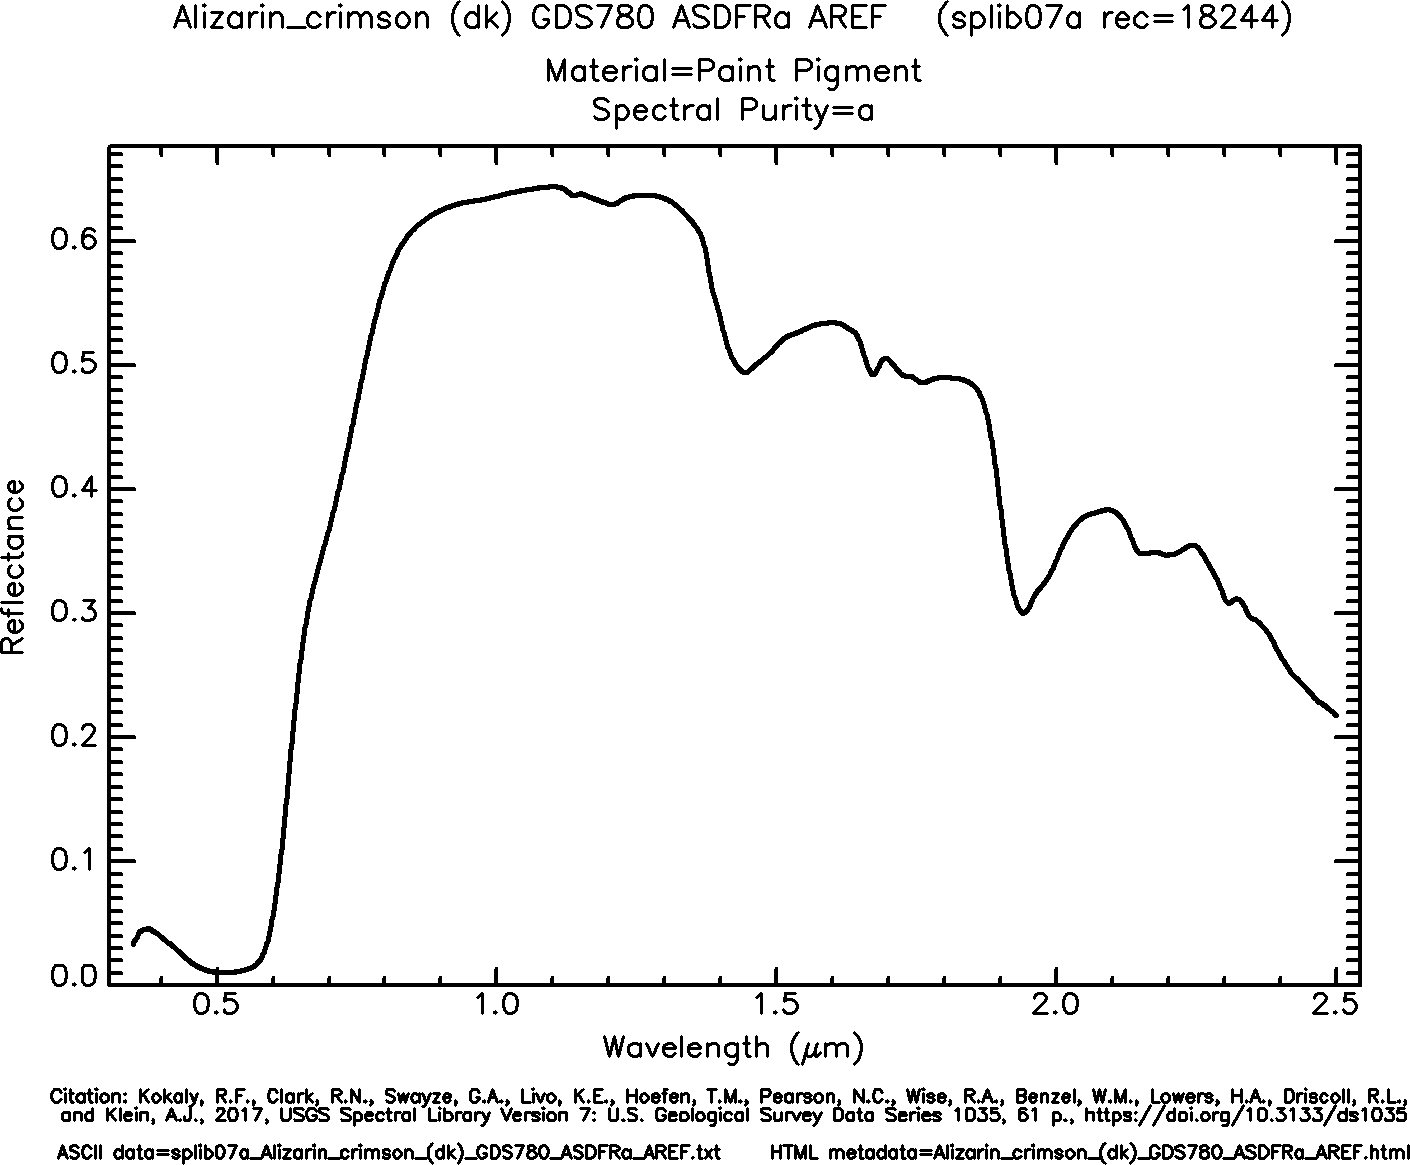
\includegraphics[width=0.8\textwidth]{esempio_firma.png}
    \caption{Firma spettrale dell'alizarina cremisi}
    \label{esempio_firma}
\end{figure}

\subsection{USGS Spectral Library}
Il dataset scelto per verificare la fattibilità della classificazione di oggetti tramite la loro firma spettrale è stato quello dello United States
Geological Survey, un'agenzia scientifica del governo degli Stati Uniti d'America.
Il dataset è denominato USGS Spectral Library Version 7.
Questo insieme di dati è stato raccolto nel corso degli anni dai ricercatori dell'ente menzionato facendo rilevazioni su migliaia di materiali in laboratorio,
usando diversi tipi di spettrometri, i quali coprono lunghezze d'onda che vanno dall'ultravioletto all'infrarosso (da \unit{0.2}{\micro\meter} a \unit{200}{\micro\meter}).
Gli strumenti usati, in dettaglio, sono:
\begin{itemize}
    \item Beckman\textsuperscript{TM} 5270, il quale copre l'intervallo spettrale dai 0.2 ai 3 \micro\meter;
    \item i modelli standard, high-resolution (hi-res) e high-resolution Next Generation (hi-resNG) della Analytical Spectral Devices (ASD);
          che coprono tutti dai 0.35 ai 2.5 \micro\meter;
    \item Nicolet\textsuperscript{TM} Fourier Transform Infra-Red (FTIR) che copre dai 1.12 ai 216 \micro\meter;
    \item NASA Airborne Visible/Infra-Red Imaging Spectrometer (AVIRIS) il quale copre dai 0.37 ai 2.5 \micro\meter.
\end{itemize}
Le classi di materiale prese in considerazione sono:
\begin{itemize}
    \item minerali;
    \item terreno (incluso rocce e minerali);
    \item rivestimenti su superfici rocciose;
    \item liquidi;
    \item composti organici;
    \item materiali artificiali;
    \item vegetazione e altri materiali biologici.
\end{itemize}
Una caratteristica degna di nota del dataset è che in corrispondenza di lunghezze d'onda il cui valore di riflettanza fosse stato eccessivamente sporcato da gas atmosferici questo è stato impostato a $-1.23 \cdot 10^{34}$, il quale corrisponde al "deleted channel" del software SPECPR (SPECtrum Processing Routines). Di conseguenza questi valori dovranno essere rimossi, per evitare che il modello prenda degli input inconsistenti durante il processo di allenamento.\\
In totale sono stati presi in considerazione 61453 esempi, con la distribuzione in classi riportata in figura \ref*{distr_esempi}. Come si può notare dal grafico, ci troviamo in presenza di dati sbilanciati.

\begin{figure}
    \centering
    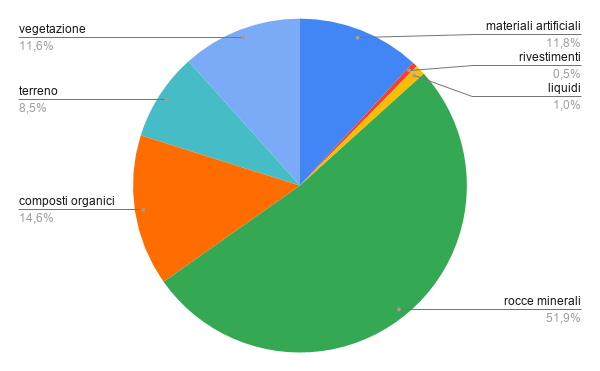
\includegraphics[width=0.8\textwidth]{distribuzione_dataset.png}
    \caption{Distribuzione esempi dataset in classi}
    \label{distr_esempi}
\end{figure}

\subsection{Elaborazione dei dati}
In primo luogo è stato necessario formattare i dati contenuti nel dataset in modo che fossero poi pronti come input per il modello di machine learning. Originariamente questi erano contenuti in file formato \verb|.txt| codificati in ASCII. In particolare erano suddivisi in cartelle in base allo spettrometro usato nelle rilevazioni e all'anno in cui sono state effettuate. Dentro ognuna di queste poi, vi era una cartella per ogni classe di materiale, contenente le lo spettro luminoso di ogni materiale. Il file con la lunghezza d'onda era comune per tutti i materiali. Per questa attività si sono realizzati degli script in linguaggio Python, i quali rimuovevano caratteri come spazi e stringhe. Il risultato, per ogni cartella, è un file \verb|data.txt| in cui ogni linea identifica una rilevazione. In particolare il primo numero intero $n \in \{ 0 .. 6 \}$ identifica la classe di appartenenza secondo questa mappa:
\begin{itemize}
    \item $0 \rightarrow$ materiali artificiali
    \item $1 \rightarrow$ rivestimenti
    \item $2 \rightarrow$ liquidi
    \item $3 \rightarrow$ rocce minerali
    \item $4 \rightarrow$ composti organici
    \item $5 \rightarrow$ terreno
    \item $6 \rightarrow$ vegetazione
\end{itemize}
Successivamente ci sono $k$ numeri che rappresentano lo spettro luminoso, seguiti da altrettanti per le lunghezze d'onda corrispondenti. Più in dettaglio, il numero n-esimo nell'array dello spettro luminoso corrisponde all'n-esimo nell'array delle lunghezze d'onda. Il valore $k$ dipende dallo strumento usato per la rilevazione.\\
Vista l'eterogeneità delle righe del file, le quali hanno lunghezze diverse a causa della diversità delle misurazioni effettuate, si è resa necessaria una fase di uniformazione. Questa è stata effettuata usando il software proprietario MATLAB\_R2021A, lo script è il seguente:

\begin{lstlisting}
    clear;
    clc;
    dataset = fopen('dataset.txt', 'r');
    y_file = fopen('y.txt', 'w');
    x_file = fopen('x.txt', 'w');

    line = fgetl(dataset);
    while ischar(line)
        % converting txt line to array
        splitted = split(line, ';');
        wavelengths = str2double(split(splitted(3), ','));
        reflectance = str2double(split(splitted(2), ','));
        
        % removing dirty channels
        idx = ismember(reflectance, 1.23e34);
        reflectance(idx) = [];
        wavelengths(idx) = [];
        
        % interpolation
        x = linspace(wavelengths(1), wavelengths(end), 2000);
        s = spline(wavelengths, reflectance, x);
        
        % writing result to files
        fprintf(y_file, '%d\n', str2double(splitted(1)));
        fprintf(x_file, '%f ',s);
        fprintf(x_file, '\n');
        
        % getting next line
        line = fgetl(dataset);
    end

    fclose(dataset);
    fclose(y_file);
    fclose(x_file);
\end{lstlisting}
dove il file \verb|dataset.txt| è l'unione dei file generati per ogni cartella in precedenza con lo script Python.
Ogni linea viene divisa nelle tre parti prima descritte, inoltre dai valori di riflettanza e lunghezza d'onda vengono rimossi i canali con valori eliminati a causa di errori troppo elevati nella rilevazione.
Successivamente i valori vengono interpolati con una spline cubica e portati ad un'unica dimensionalità di 2000 punti. Quello che interessa per identificare un oggetto tramite la firma spettrale, cosi come dedotto dall'incontro con l'esperto in geologia, è l'andamento del valore di riflettanza, ad esempio particolari picchi o oscillazioni. Di conseguenza non è fondamentale che i valori di lunghezza d'onda siano esattamente gli stessi, perciò l'interpolazione avviene considerando gli estremi dell'intervallo delle lunghezze d'onda per ogni esempio. È stato scelto questo particolare metodo di interpolazione visto che assicura la convergenza anche con nodi equispaziati ed è stabile, al contrario di quello polinomiale.\\
L'output di questo script sono i due file \verb|x.txt| e \verb|y.txt|, i quali sono pronti ad essere caricati in linguaggio Python per usarli come input del modello di apprendimento automatico.

\section{Sviluppo del modello di machine learning}
Tra le varie possibilità che i framework per i machine learning offrono al giorno d'oggi si sono fatte alcune considerazioni sui seguenti, facendo ricadere la scelta finale sulle reti neurali MLP (Multi-Layer-Perceptron).

\subsection{Strumento adottato}
Per questa parte del progetto ci si è affidati allo strumento offerto as-a-service Google Colaboratory, il quale è un'implementazione del progetto Jupyter con base di archiviazione Google Drive.
I Jupyter notebook sono un'insieme di script python intervallati da testo descrittivo.
Il vantaggio nell'utilizzo di questo strumento è innanzitutto la possibilità di usare hardware come GPU offerte gratuitamente dall'infrastruttura cloud di Google per eseguire gli script. Inoltre è possibile eseguire una parte di codice alla volta o tutto insieme, mantenendo le variabili in memoria RAM per tutta la durata della sessione. È possibile quindi allenare la rete e successivamente eseguire dei test sul modello allenato, stampare grafici con le curve di apprendimento o salvare il modello allenato su Google Drive.

\subsection{Scelta del modello}
\subsubsection{k-nearest-neighbour}
Una prima considerazione è stata fatta in base al successivo utilizzo del modello allenato: questo dovrà essere interpellato per effettuare predizioni in real time, dunque il tempo di risposta dovrà essere costante. Ne segue che modelli basati su \textbf{k-nearest-neighbour} non possono essere adottati, in quanto il tempo di esecuzione dell'algoritmo di predizione ricade nella classe di complessità $\theta (n)$ dove $n$ è il numero di esempi classificati. Questo perché la classificazione dei nuovi esempi si basa sul calcolo della distanza dagli esempi nel training set in uno spazio d-dimensionale (dove $d$ è il numero di features, nel nostro caso 2000), successivamente si trovano i $k$ esempi più vicini a quello da classificare, tra questi si guarda la classe più frequente. Una volta che un esempio è classificato viene usato nelle predizioni successive, dunque il tempo per il calcolo delle distanze aumenta. Questo è impraticabile in un sistema real-time, il quale richiede che i tempi di risposta siano costanti, ne segue la decisione prima menzionata.

\subsubsection{Support Vector Machines}
Questo tipo di modello è stato preso in considerazione visto che è un algoritmo di apprendimento supervisionato usato spesso per compiti di classificazione. È un modello di classificazione lineare ma può essere usato efficientemente per effettuare classificazioni non lineari usando il \textit{kernel trick}. Inoltre è molto efficace in spazi a molte dimensioni.
Per l'implementazione ci si è affidati alla libreria scikit-learn, la quale offre dei modelli per la classificazione con le seguenti classi:
\begin{itemize}
    \item SVC: Support Vector Classification, la cui implementazione è basata sulla libreria \verb|libsvm| scritta in linguaggio C++, dunque offre la velocità di un linguaggio compilato. Il tempo di training è nella classe di complessità $\theta (n^2)$ con $n$ il numero di esempi nel set di training, dunque diventa inutilizzabile con le dimensioni del nostro dataset. Questo perché effettua un tipo di classificazione one-vs-one, dunque allena $k \cdot (k-1)/2$ classificatori binari con $k$ il numero di classi;
    \item NuSVC: simile al precedente ma aggiunge un parametro per controllare il numero dei support vectors;
    \item LinearSVC: questo è stato il tipo di modello che si è provato ad utilizzare nel nostro caso. A differenza dei precedenti allena dei classificatori di tipo one-vs-all, ovvero un classificatore per ogni classe. Ne segue che non c'è più la complessità quadratica per l'algoritmo di allenamento. È simile alla classe SVC con parametro nel costruttore \verb|kernel='linear'|, tuttavia la sua implementazione si basa sulla libreria \verb|liblinear|, anch'essa scritta in C++ ma che scala meglio all'aumentare delle dimensioni del dataset.
\end{itemize}
Il modello è stato inserito in una pipeline che prevedesse uno step precedente per la normalizzazione delle features tramite la classe \verb|StandardScaler| offerta dalla stessa libreria. Si è applicata inoltre la procedura di hold-out, che prevede la suddivisione del dataset in due parti, training e validation set. La dimensione scelta per il primo è $80\%$, per il secondo il restante $20\%$, la suddivisione è stata effettuata in modo casuale usando la funzione \verb|train_test_split| offerta dalla stessa libreria.\\
Successivamente il modello allenato è stato testato valutando l'accuratezza nell'effettuare le predizioni sul set di validazione, le prove hanno dato esito negativo visto che non si è superato il $62\%$ in questa metrica.

\subsubsection{Multi Layer Perceptron}
In seguito all'insuccesso riportato con le Support Vector Machines con kernel lineare si è deciso di passare ad algoritmi di deep learning. Si sono prese in considerazione le classiche rete neurali artificiali a strati, adottando la libreria Pytorch per l'implementazione, visto che permette di addestrare la rete su GPU rendendo questo processo significativamente più veloce.
L'unità fondamentale in questo tipo di modello è il percettrone (neurone), il quale rappresenta un modello di machine learning semplice, dotato di una funzione e di un valore di attivazione. Ogni unità è connessa a tutte quelle nello strato successivo e ad ogni connessione è associato un peso (appreso tramite backpropagation). Ad ogni strato è inoltre associato un bias. Per calcolare il valore di attivazione di ogni neurone si effettua un'operazione lineare che vede la somma tra il valore di attivazione del neurone nel layer precedente moltiplicato per il peso della connessione, a cui si somma infine il bias del layer (anch'esso appreso automaticamente). Questo è definito passo di forward, l'idea di funzionamento viene meglio presentata nell'algoritmo \ref*{grad_desc_backprop}.\\
Il layer di output sarà composto da 7 percettroni, ognuno dei quali indica la probabilità che un certo esempio appartenga o meno alla classe rappresentata (infatti nel dataset ci sono 7 classi di oggetti).

\begin{algorithm}
    \caption{Gradient descent with backpropagation}
    \label{grad_desc_backprop}
    \begin{algorithmic}
        \State Training samples $\{ (x^{(1)}, y^{(1)}), \dotso, (x^{(m)}, y^{(m)}) \}$
        \State Initialize $\theta^{l}$ with random values close to zero, e.g. $\in [-\epsilon, +\epsilon]$
        \For{all epochs}
            \State Initialize $\Delta_{ij}^{(l)} = 0$ $\forall i, j, l$ \Comment Accumulatori per calcolo derivata
            \For{k=1 to m}
                \State set $a^{(1)} = x^{(k)}$ \Comment imposto primo layer da input
                \For{l=2 to L}
                    \State compute $a^{(l)}$ \Comment forward propagation
                \EndFor
                \State compute $\delta^{(L)} = a^{(L)} - y^{(k)}$
                \For{l=L-1 down to 2}
                    \State compute $\delta^{(l)} = ((\theta^{(l)})^T \cdot \delta^{l+1}) \ .* f'(z^{l})$ \Comment backpropagation
                \EndFor
                \State compute gradients $\Delta^{(l)} = \Delta^{(l)} + \delta^{(l+1)} \cdot (a^{(l)})^T$
            \EndFor
            \State compute $D^{(l)}_{ij} = 
            \begin{cases}
                \frac{1}{m} \cdot (\Delta^{(l)}_{ij} + \lambda \theta^{(l)}_{ij}) \ \ if \ \ j \neq 0 \\
                \frac{1}{m} \cdot \Delta^{(l)}_{ij} \ \ if \ \ j = 0
            \end{cases}$
            \State $\theta^{(l)}_{ij} = \theta^{(l)}_{ij} - \eta \cdot D_{ij}^{(l)}$
        \EndFor
    \end{algorithmic}
\end{algorithm}

\subsection{Implementazione e validazione}
Come prima accennato, si è fatto largo uso di Pytorch nell'implementazione della rete. In particolare si è definita la classe \verb|MLP| che eredita da \verb|nn.Module|, ovvero la classe base per ogni modello di rete neurale. Non sono stati ridefiniti metodi degni di nota, se non la possibilità di invocare il costruttore modificando gli iperparametri della rete in modo semplice. Inoltre si è adottata la variante Adam di gradient descent, che assicura una convergenza più veloce. Gli iperparametri adottati sono i seguenti:
\begin{itemize}
    \item \verb|layers size:| $[2000, 1500, 500, 7]$, indica il numero di neuroni per ogni layer. In questo caso abbiamo una rete a 3 strati (2 nascosti e uno di output);
    \item \verb|activation:| come funzione di attivazione dei neuroni si è scelta la funzione rectifier (ReLU) definita come $f(x) = x^+ = max(0,x)$ (vedi figura \ref*{relu_func});
    \begin{figure}
        \centering
        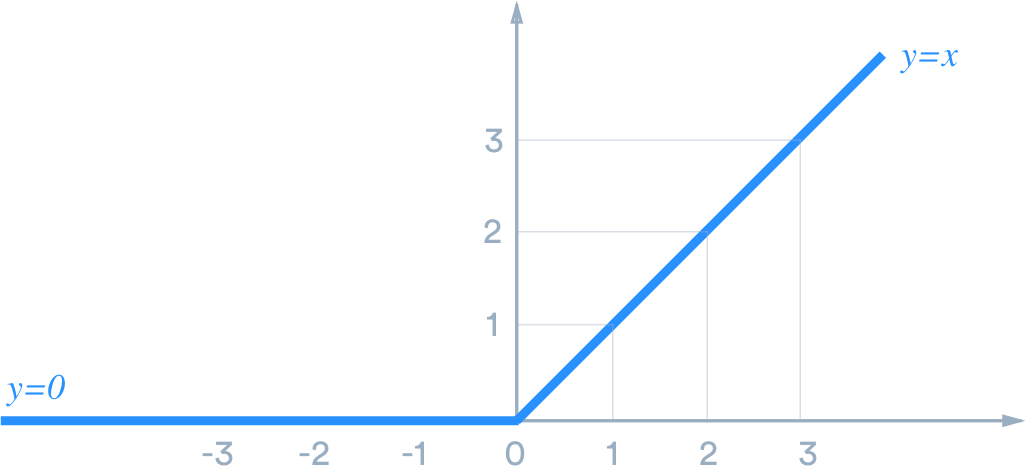
\includegraphics[width=0.6\textwidth]{relu.png}
        \caption{Funzione ReLU}
        \label{relu_func}
    \end{figure}
    \item \verb|learning rate:| $10^{-4}$, questo è il parametro $\eta$ usato in gradient descent. Se troppo basso l'algoritmo diventa lento, se troppo alto si rischia di fare overshooting (saltare il minimo della funzione di costo) o addirittura divergere;
    \item \verb|epochs:| 50, indica il numero di epoche nell'algoritmo di apprendimento;
    \item \verb|init kind:| xavier, indica come inizializzare i pesi $\theta$ delle connessioni tra i neuroni;
    \item \verb|dropout rate:| 0.2 indica che il $20\%$ dei neuroni viene disattivato scegliendo casualmente. È un tipo di regolarizzazione e serve a ridurre overfitting.
\end{itemize}
Le prestazioni ottenute con i parametri sopra elencate sono riportate nelle figure \ref*{cross_entropy_loss_plot} e \ref*{accuracy_plot}. 

\begin{figure}
    \centering
    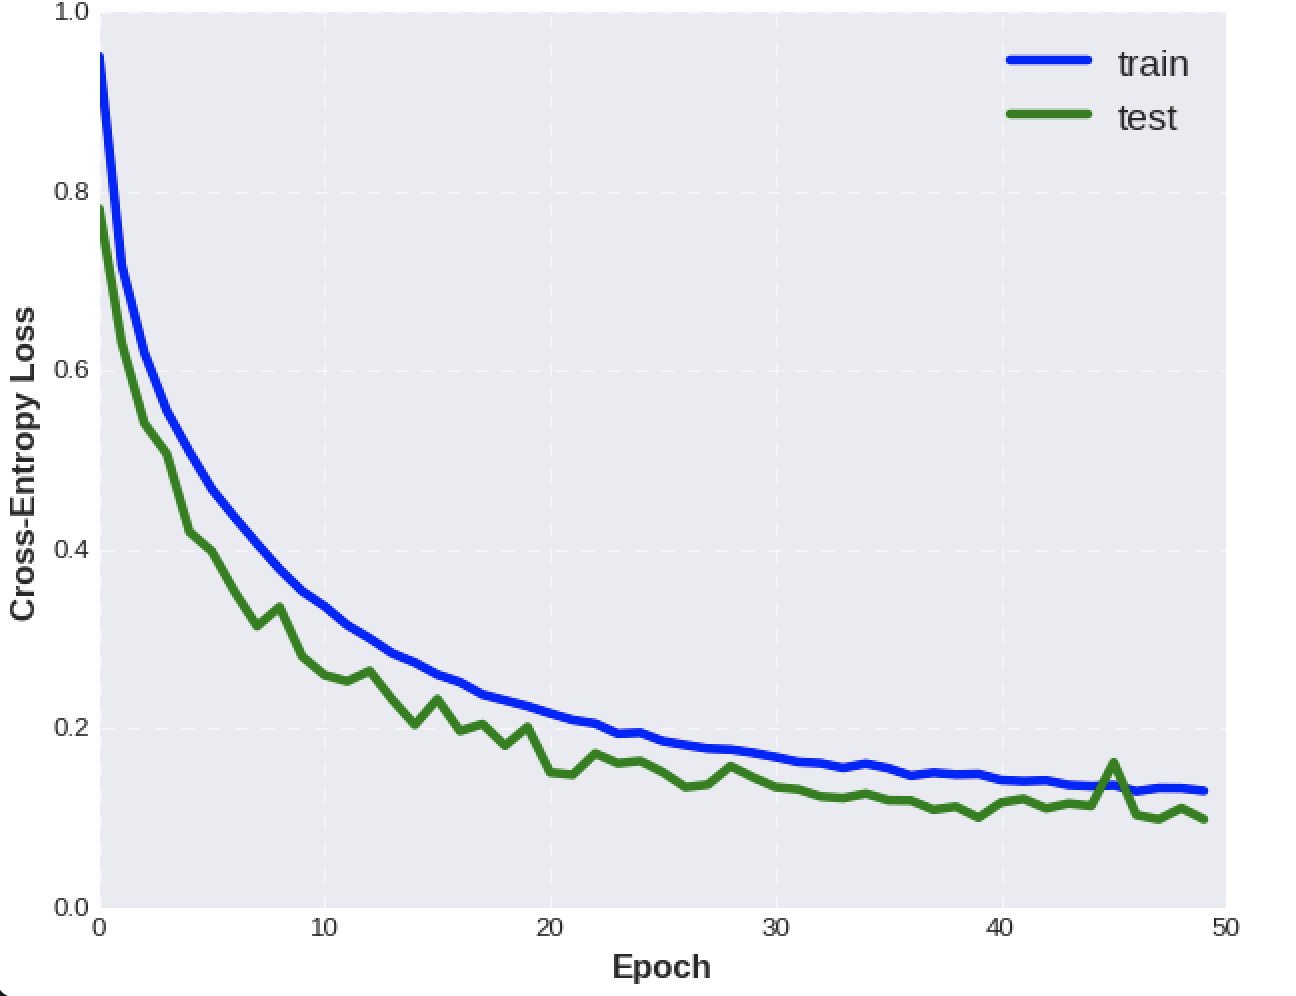
\includegraphics[width=0.9\textwidth]{cross_entropy_loss.png}
    \caption{Cross Entropy Loss plot}
    \label{cross_entropy_loss_plot}
\end{figure}

\begin{figure}
    \centering
    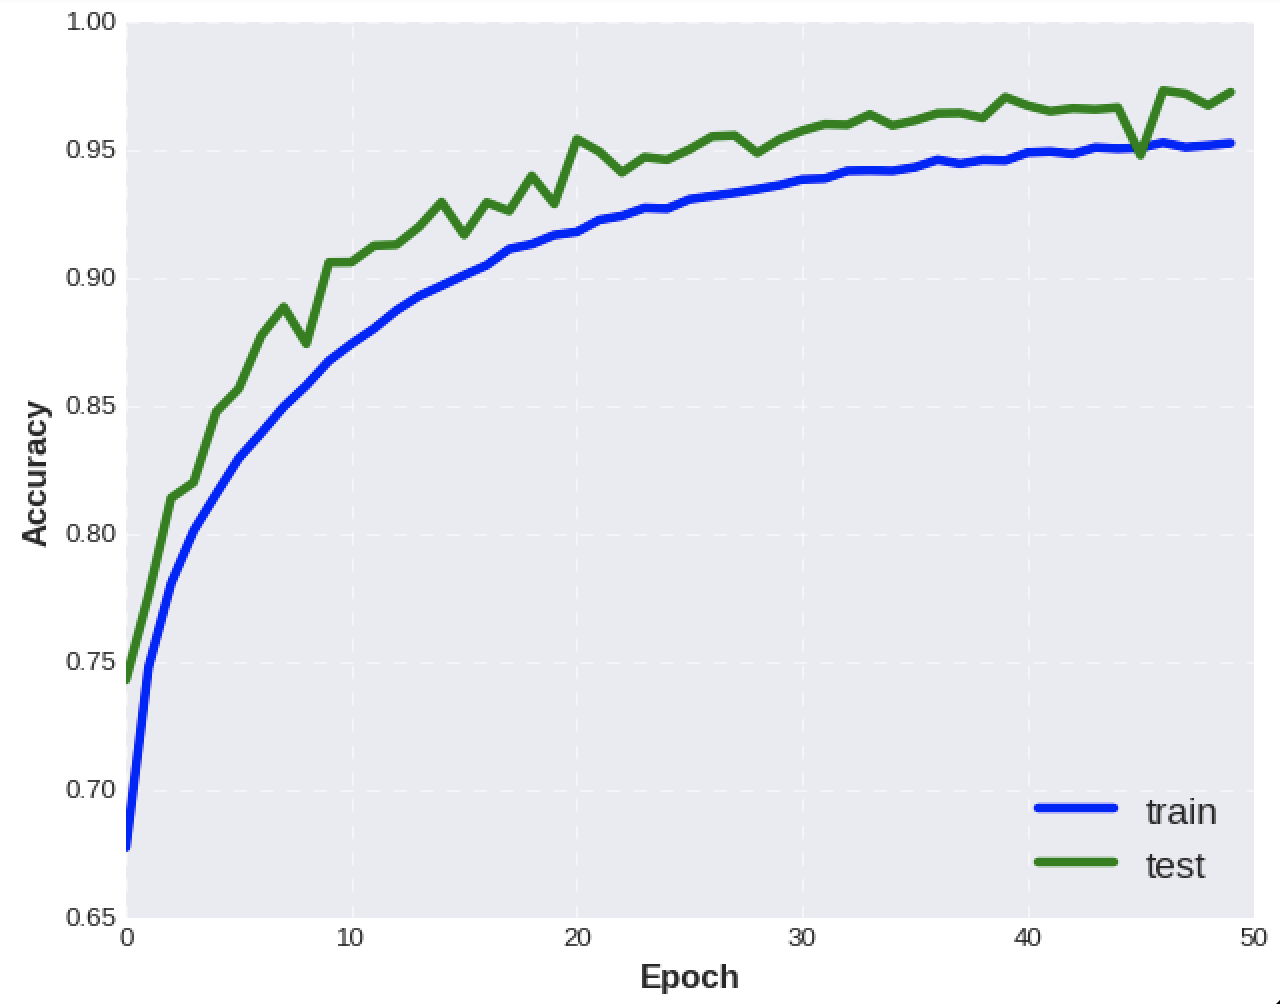
\includegraphics[width=0.9\textwidth]{accuracy.png}
    \caption{Accuracy plot}
    \label{accuracy_plot}
\end{figure}
Nella prima si vede come la funzione di costo diminuisca con l'avanzare delle epoche di apprendimento, nella seconda si può notare l'aumentare dell'accuratezza anche nel set di test.\\
Il dataset è stato suddiviso in tre insiemi disgiunti:
\begin{itemize}
    \item training set: usato per la fase di apprendimento è composto dal $70\%$ degli esempi;
    \item test set: usato nella fase di apprendimento per verificate l'andamento alla fine di ogni epoca, è composto dal $15\%$ degli esempi;
    \item validation set: usato alla fine della fase di apprendimento per valutare le prestazioni del modello allenato, è composto dal restante $15\%$ degli esempi.
\end{itemize}
Come si può notare dal grafico \ref*{accuracy_plot}, il valore di accuratezza raggiunto alla cinquantesima epoca è intorno al $97\%$. I risultati di predizione sul set di validazione mostrano un'accuratezza del $98.23\%$, per un totale di 9055 esempi su 9218 classificati correttamente.
